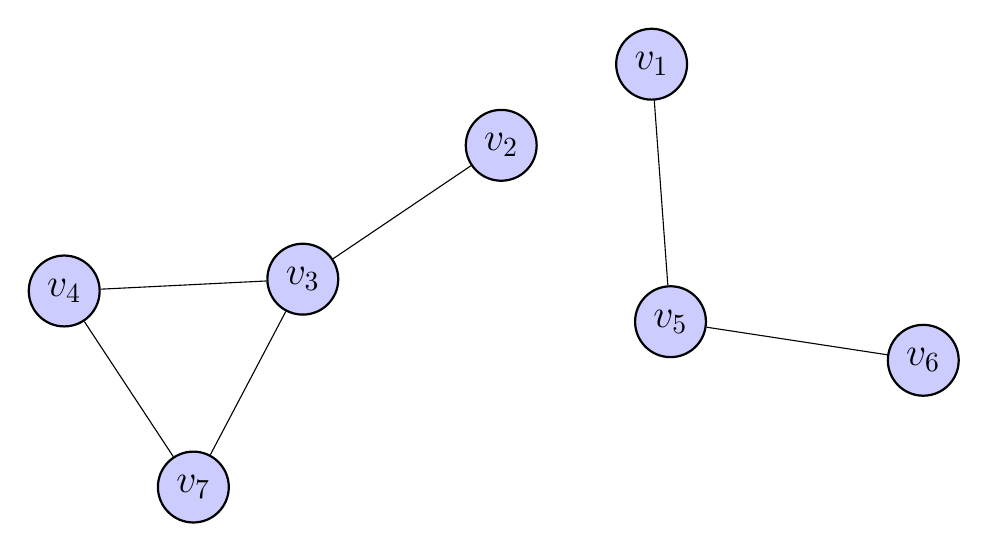
\begin{tikzpicture}[
  scale=1,
  vnode/.style={circle, fill=blue!20, draw=black, thick, minimum size=9mm, inner sep=0pt, font=\Large}
]
  % Vértices
  \node[vnode] (v1) at (7.85, 6.82) {$v_1$};
  \node[vnode] (v2) at (5.94, 5.79) {$v_2$};
  \node[vnode] (v3) at (3.42, 4.09) {$v_3$};
  \node[vnode] (v4) at (0.39, 3.94) {$v_4$};
  \node[vnode] (v5) at (8.09, 3.55) {$v_5$};
  \node[vnode] (v6) at (11.30, 3.06) {$v_6$};
  \node[vnode] (v7) at (2.03, 1.45) {$v_7$};

  % Aristas
  \foreach \from/\to in {v1/v5, v2/v3, v3/v4, v3/v7, v4/v7, v5/v6}
    \draw (\from) -- (\to);
\end{tikzpicture}
